\documentclass[aspectratio=169,11pt]{beamer}

\usetheme{Madrid}
% \setbeamertemplate{frametitle}{%
%   \nointerlineskip
%   \begin{beamercolorbox}[
%     sep=0.3cm,
%     wd=\paperwidth,
%     ht=0.9cm,
%     dp=0.25cm
%   ]{frametitle}
%     \usebeamerfont{frametitle}%
%     \insertframenumber.\hspace{0.3em}\insertframetitle
%   \end{beamercolorbox}
% }
\setbeamertemplate{navigation symbols}{}
\setbeamertemplate{footline}[frame number]

\usepackage{comment}
\usepackage{amsmath,amssymb}
\usepackage{booktabs}
\usepackage{graphicx}
\usepackage{xcolor}
\usepackage{listings}
\usepackage{array}
\usepackage{booktabs}
\usepackage{tikz}
\usetikzlibrary{positioning,arrows.meta}
\usepackage{tabularx}

\definecolor{codebg}{RGB}{245,245,245}
\lstset{
  basicstyle=\ttfamily\scriptsize,
  backgroundcolor=\color{codebg},
  frame=single,
  breaklines=true,
  showstringspaces=false,
  columns=fullflexible
}

\newcommand{\figureplaceholder}[2][0.92\textwidth]{%
  \begin{center}
  \fbox{\parbox[c][3.0cm][c]{#1}{\centering\textit{FIGURE PLACEHOLDER}\\[0.3em]#2}}
  \end{center}
}

\newcommand{\smallplaceholder}[1]{%
  \begin{center}
  \fbox{\parbox[c][1.6cm][c]{0.95\linewidth}{\centering\scriptsize\textit{FIGURE PLACEHOLDER}\\#1}}
  \end{center}
}
\lstset{
    basicstyle=\ttfamily\tiny,
    frame=single,
    columns=fullflexible,
    keepspaces=true,
    showstringspaces=false,
    aboveskip=2pt,
    belowskip=2pt,
    xleftmargin=2pt,
    framexleftmargin=2pt
}
\title{Continual Multi-Task Test-Time Adaptation}
\subtitle{Understanding and Mitigating Negative Transfer in Long-Term Adaptation.
}
% \date{Lab Meeting}

\begin{document}

% -----------------------------------------------------------------------------
\begin{frame}
% [noframenumbering]
  \titlepage
\end{frame}

% -----------------------------------------------------------------------------
\begin{frame}{1. Motivation: Why Multi-Task CTTA?}

\begin{columns}[T]
\column{0.48\textwidth}
\textbf{Most CTTA methods are single-task}
\begin{itemize}
  \item Adapt one prediction task in isolation.
  \item Pseudo-supervision comes from the same task being adapted.
\end{itemize}

\textbf{Autonomous driving is multi-task}
\begin{itemize}
  \item Object detection: object existence, class, geometry.
  \item Semantic segmentation: dense pixel-level semantics.
  \item Both share the same visual representation.
\end{itemize}

\column{0.48\textwidth}
% \smallplaceholder{Example target frame with detection boxes + semantic map}

\vspace{0.3em}
\begin{block}{Research question}
Can the two tasks help each other during continual adaptation without amplifying errors through the shared representation?
\end{block}
\end{columns}
\end{frame}

% -----------------------------------------------------------------------------
\begin{frame}{2. Problem Setting}
\begin{itemize}
  \item \textbf{Source:} Cityscapes.
  \item \textbf{Model:} Panoptic-FPN R50-FPN.
  \item \textbf{Tasks:} 8-class detection + 19-class semantic segmentation.
  \item \textbf{Strict online CTTA:} batch size 1, each image seen once, no target labels, no reset.
\end{itemize}

\vspace{0.5em}
\begin{columns}[T]
\column{0.48\textwidth}
\textbf{Short-term}
\begin{itemize}
  \item ACDC4: fog, night, rain, snow
  \item CSC12: 12 Cityscapes-C corruptions
\end{itemize}

\column{0.48\textwidth}
\textbf{Long-term}
\begin{itemize}
  \item ACDC-LT: 4 domains $\times$ 10 rounds
  \item CSC-LT: 5 corruptions $\times$ 10 rounds
\end{itemize}
\end{columns}
\end{frame}

% -----------------------------------------------------------------------------
\begin{frame}{3. Source Multi-Task Architecture}
\begin{itemize}
  \item Shared ResNet-50 backbone.
  \item Shared FPN.
  \item Faster R-CNN-style detection branch.
  \item Semantic segmentation branch.
\end{itemize}

\begin{figure}
    \centering
    \includegraphics[
        width=0.6\textwidth,
        height=0.6\textheight,
        keepaspectratio
    ]{figures/panoptic_fpn.png}
\end{figure}

\end{frame}

% -----------------------------------------------------------------------------
\begin{frame}{4. Base Multi-Task CTTA Framework}
\begin{columns}[T]
\column{0.48\textwidth}
\textbf{Student}
\begin{itemize}
  \item Adapted online.
  \item Joint detection + segmentation model.
\end{itemize}

\textbf{EMA Teacher}
\begin{itemize}
  \item Generates detection pseudo-labels.
  \item Generates semantic soft targets.
\end{itemize}

\textbf{Frozen Source Anchor}
\begin{itemize}
  \item Never updated.
  \item Provides confidence for conditional teacher-target selection.
\item Provides source-marginal KL stabilization.
\item Source parameters for stochastic restoration.
\end{itemize}

\column{0.48\textwidth}

\begin{figure}
    \centering
    \includegraphics[
        width=\linewidth,
height=0.68\textheight,
keepaspectratio
    ]{figures/method.png}
\end{figure}


\end{columns}
\end{frame}

% -----------------------------------------------------------------------------
\begin{frame}[fragile]{5. Online Adaptation: Per-Frame Update}
For each incoming unlabeled target image $x_t$:

\begin{enumerate}
  \item Teacher inference.
  \item Detection pseudo-label construction.
  \item Score-EMA detection reliability gate.
  \item Student forward on a strong view.
  \item Compute detection, semantic, and anchor losses.
  \item Student SGD update.
  \item EMA teacher update.
  \item Stochastic source restoration.
\end{enumerate}

\begin{block}{Base adaptation objective}
\[
\mathcal{L}_{\mathrm{Base}}
=
\mathcal{L}_{\mathrm{det}}
+
\mathcal{L}_{\mathrm{seg}}
+
0.1\,\mathcal{L}_{\mathrm{anchor}}
\]
\end{block}

\begin{lstlisting}[basicstyle=\ttfamily\tiny,aboveskip=2pt,belowskip=0pt]
pseudo_det, q_t = teacher_targets(x_t)
optimizer.zero_grad()
loss.backward()
optimizer.step()
update_ema_teacher()
stochastic_restore(student)
\end{lstlisting}

\end{frame}

% -----------------------------------------------------------------------------
\begin{frame}{6. Object Detection Adaptation}
\textbf{AMROD-inspired teacher pseudo-supervision}

\begin{itemize}
  \item Dynamic class-specific confidence thresholds.
  \item NMS + pseudo-label filtering.
  \item Standard Faster R-CNN losses on accepted teacher boxes.
  \item Score-EMA gate can suppress unreliable detection adaptation only.
\end{itemize}
\vspace{-0.5cm}

\[
\mathcal{L}_{\mathrm{det}}
=
\mathcal{L}_{\mathrm{RPN\text{-}cls}}
+
\mathcal{L}_{\mathrm{RPN\text{-}box}}
+
\mathcal{L}_{\mathrm{ROI\text{-}cls}}
+
\mathcal{L}_{\mathrm{ROI\text{-}box}}
\]
% \vspace{-1cm}
{\scriptsize
Standard Faster R-CNN classification and box-regression losses,
using accepted teacher detections as pseudo ground truth.
}
\[
\tau_{c,t}=\operatorname{clip}_{[0.70,0.80]}
\left[\gamma\tau_{c,t-1}+(1-\gamma)\alpha\sqrt{\bar{s}_{c,t}}\right],
\quad \alpha=1.3,\;\gamma=0.95
\]
% \vspace{-0.5cm}
\begin{figure}
    \centering
    \includegraphics[
        width=0.6\textwidth,
        height=0.4\textheight,
        keepaspectratio
    ]{figures/object_detection.png}
\end{figure}


\end{frame}

% -----------------------------------------------------------------------------
% % \begin{frame}{7. Semantic Segmentation Adaptation}

% % \begin{columns}[T,onlytextwidth]

% % % =========================================================
% % % LEFT COLUMN
% % % =========================================================
% % \begin{column}{0.53\textwidth}

% % \small

% % \begin{itemize}
% %   \setlength{\itemsep}{2pt}
% %   \item Soft teacher--student consistency.
% %   \item Strong student view.
% %   \item Class-balanced supervision.
% %   \item Conditional augmentation-averaged teacher target.
% %   \item Frozen source-anchor marginal KL. Anchor KL is applied to image-level semantic class marginals, not pixel-wise predictions.
% % \end{itemize}

% % \vspace{-0.35cm}

% % \[
% % \mathcal{L}_{\mathrm{seg}}
% % =
% % -\frac{1}{HW}
% % \sum_{i=1}^{HW}
% % \sum_{k=1}^{K}
% % w_{k,t}\,
% % q^T_{i,k}
% % \log p^S_{i,k}
% % \]

% % \vspace{-0.25cm}

% % {\scriptsize
% % Class weights $w_{k,t}$ are normalized to preserve the
% % overall loss scale.
% % }

% % \vspace{-0.35cm}

% % \[
% % \mathcal{L}_{\mathrm{anchor}}
% % =
% % D_{\mathrm{KL}}
% % \!\left(
% % q^{A}\parallel p^{S}
% % \right)
% % \]

% % \end{column}


% % % =========================================================
% % % RIGHT COLUMN
% % % =========================================================
% % \begin{column}{0.5\textwidth}

% % \centering

% % \vspace{0.4cm}

% % \includegraphics[
% %     width=\linewidth,
% %     height=0.68\textheight,
% %     keepaspectratio, trim=0.5cm 0.5cm 0.5cm 0.5cm,
% %     clip
% % ]{figures/semantic_segm.png}

% % \end{column}

% % \end{columns}

% \end{frame}

\begin{frame}{7. Semantic Segmentation Adaptation}

\fontsize{6.8}{7.3}\selectfont

\setlength{\abovedisplayskip}{1pt}
\setlength{\belowdisplayskip}{1pt}
\setlength{\abovedisplayshortskip}{1pt}
\setlength{\belowdisplayshortskip}{1pt}
\setlength{\jot}{0.5pt}

% \vspace{-0.18cm}

% =========================================================
% TOP: PIPELINE FIGURE
% =========================================================
\vspace{-0.3cm}

\begin{center}
\includegraphics[
    width=0.88\textwidth,
    height=0.55\textheight,
    keepaspectratio,
    trim=0.2cm 0.8cm 0.01cm 0.9cm,
    clip
]{figures/semantic_segm.png}
\end{center}

\vspace{-0.3cm}

% =========================================================
% BOTTOM: THEORY IN TWO COLUMNS
% =========================================================

\begin{columns}[T,onlytextwidth]

% ---------------------------------------------------------
% LEFT COLUMN
% ---------------------------------------------------------
\begin{column}{0.49\textwidth}

\begin{itemize}
  \setlength{\itemsep}{-1.5pt}
  \setlength{\parskip}{0pt}
  \setlength{\parsep}{0pt}
  \setlength{\topsep}{0pt}

  \item Soft teacher--student consistency.
  \item Strong student view.
  \item Class-balanced pixel supervision.
  \item Conditional augmentation-averaged teacher target.
  \item Frozen source-anchor stabilization through image-level semantic marginals.
\end{itemize}

\vspace{-0.13cm}

\textbf{Semantic consistency loss}

\vspace{-0.08cm}

For each pixel $i$:

\vspace{-0.5cm}

\[
\ell^{\mathrm{seg}}_i
=
-\sum_{k=1}^{K}
q^T_{i,k}\log p^S_{i,k},
\qquad
c_i^\ast=\arg\max_k q^T_{i,k}.
\]

\vspace{-0.10cm}

{\fontsize{5.6}{6.0}\selectfont
Soft cross-entropy between the EMA-teacher distribution
$q^T_i$ and the student prediction $p^S_i$.
The pseudo-class $c_i^\ast$ is used to assign the corresponding
class-balancing weight.
}

\end{column}


% ---------------------------------------------------------
% RIGHT COLUMN
% ---------------------------------------------------------
\begin{column}{0.49\textwidth}

\textbf{Class-balanced semantic objective}

% \vspace{-0.08cm}

\[
\mathcal{L}^{\mathrm{cb}}_{\mathrm{seg}}
=
\frac{
\sum_i w_{c_i^\ast,t}\,
\ell^{\mathrm{seg}}_i
}{
\sum_i w_{c_i^\ast,t}+\epsilon
},
\qquad
\mathcal{L}_{\mathrm{seg}}
=
\kappa_t
\mathcal{L}^{\mathrm{cb}}_{\mathrm{seg}}.
\]

% \vspace{-0.10cm}

{\fontsize{5.5}{5.9}\selectfont
Class weights are derived from running teacher class marginals.
$\kappa_t$ is a stop-gradient rescaling term that preserves the
scalar loss scale of the unweighted semantic objective.
}

% \vspace{-0.06cm}

\textbf{Source-anchor stabilization}

\vspace{-0.3cm}

\[
\mathcal{L}_{\mathrm{anchor}}
=
D_{\mathrm{KL}}
\!\left(
q_A\parallel q_S
\right).
\]

% \vspace{-0.12cm}
% 
{\fontsize{5.5}{5.9}\selectfont
$q_A$ and $q_S$ are the image-level semantic class marginals of the
frozen source anchor and the student, respectively.
}

\end{column}

\end{columns}

\end{frame}
% -----------------------------------------------------------------------------
\begin{frame}{8. Cross-Task Mechanisms Explored}

\begin{columns}[T,onlytextwidth]

% ---------------------------------
% LEFT COLUMN
% ---------------------------------
\begin{column}{0.53\textwidth}

\centering
\renewcommand{\arraystretch}{1.25}

\resizebox{\linewidth}{!}{%
\begin{tabular}{lccc}
\toprule
\textbf{Mechanism} & \textbf{Direction} & \textbf{Level} & \textbf{Goal} \\
\midrule
CT-CL & Det $\leftrightarrow$ Seg & Features & Representation alignment \\
CT-CR & Det $\rightarrow$ Seg & Pixels & Dense semantic supervision \\
CTPV  & Seg $\rightarrow$ Det & Pseudo-labels & Detection verification \\
\bottomrule
\end{tabular}
}

\vspace{0.65cm}

\begin{block}{Idea}
\small
The same physical object is observed through complementary task views.
We explored three different ways of exploiting that structure.
\end{block}

\end{column}

% ---------------------------------
% RIGHT COLUMN
% ---------------------------------
\begin{column}{0.44\textwidth}

\centering
\vspace{0.15cm}

\includegraphics[
    width=\linewidth,
    height=0.70\textheight,
    keepaspectratio
]{figures/ct_modules.png}

\end{column}

\end{columns}

\end{frame}% -----------------------------------------------------------------------------
\begin{frame}[fragile]{9. CT-CL: Cross-Task Contrastive Learning}

\scriptsize
\setlength{\abovedisplayskip}{3pt}
\setlength{\belowdisplayskip}{3pt}
\setlength{\abovedisplayshortskip}{2pt}
\setlength{\belowdisplayshortskip}{2pt}

\begin{columns}[T,onlytextwidth]

% ------------------------------------------------
% LEFT COLUMN
% ------------------------------------------------
\begin{column}{0.57\textwidth}

\begin{itemize}
  \setlength{\itemsep}{0pt}
  \setlength{\parskip}{0pt}
  \setlength{\parsep}{0pt}
  \item Detection embedding for each pseudo-object.
  \item Semantic embedding over the same region.
  \item Same-class cross-task pairs: positives.
  \item Different-class pairs: negatives.
\end{itemize}

\vspace{0.05cm}

For pseudo-object $(b,c)$:

\[
\begin{aligned}
z_{\mathrm{det}}
&=
\phi_{\mathrm{det}}
\!\left(\mathrm{RoIAlign}(F^S,b)\right),
\\[1pt]
z_{\mathrm{seg}}
&=
\phi_{\mathrm{seg}}
\!\left(
\frac{\sum_{p\in b}q_T(p,\sigma(c))F^S_p}
{\sum_{p\in b}q_T(p,\sigma(c))+\epsilon}
\right).
\end{aligned}
\]

\vspace{-0.05cm}

{\tiny
\[
\mathcal{L}_{\mathrm{CTCL}}
=
-\sum_i\frac{1}{|P(i)|}
\sum_{p\in P(i)}
\log
\frac{e^{z_i^\top z_p/\tau}}
{\sum_{a\neq i}e^{z_i^\top z_a/\tau}}
\]
}

\vspace{0.1cm}

\begin{lstlisting}[
basicstyle=\ttfamily\tiny,
aboveskip=1pt,
belowskip=1pt,
lineskip=-1pt
]
for box, cls in pseudo_objects:
    z_det = roi_embed(F, box)
    s = det_to_sem(cls)
    w = q_teacher[box, s]
    z_seg = weighted_pool(F[box], w)
    Z += [z_det, z_seg]
    Y += [cls, cls]

L_CTCL = supcon(Z, Y)
\end{lstlisting}

\end{column}

% ------------------------------------------------
% RIGHT COLUMN
% ------------------------------------------------
\begin{column}{0.41\textwidth}

\centering

\includegraphics[
    width=1.5\linewidth,
    height=0.70\textheight,
    keepaspectratio
]{figures/ctcl.png}

\vspace{0.1cm}

\begin{block}{Hypothesis}
\tiny
Feature-level alignment should make the shared representation useful
for both tasks.
\end{block}

\vspace{-0.1cm}

{\tiny
\textit{Explored mechanism; not retained in the final configuration.}
}

\end{column}

\end{columns}

\end{frame}
% -----------------------------------------------------------------------------


\begin{frame}[fragile]{10. CT-CR: Cross-Task Consistency Regularization}

% Slightly more compact than \scriptsize
\fontsize{7.2}{7.8}\selectfont

\setlength{\abovedisplayskip}{1.5pt}
\setlength{\belowdisplayskip}{1.5pt}
\setlength{\abovedisplayshortskip}{1pt}
\setlength{\belowdisplayshortskip}{1pt}
\setlength{\jot}{1pt}

\vspace{-0.15cm}

\begin{columns}[T,onlytextwidth]

% ------------------------------------------------
% LEFT COLUMN
% ------------------------------------------------
\begin{column}{0.58\textwidth}

Teacher detection provides \textbf{class, approximate location,
and spatial support}. Detection class $c$ is mapped to semantic class
$\sigma(c)$.

\vspace{-0.02cm}

For each pixel $p$ inside detection box $b$:

\vspace{-0.08cm}

\[
\begin{aligned}
y^{\mathrm{CTCR}}_p &= \sigma(c),\\[-1mm]
w_p &= \omega_{\min}
      +(1-\omega_{\min})\,q_T(p,\sigma(c)),
\end{aligned}
\]

\vspace{-0.08cm}

with $\omega_{\min}=0.2$.

\vspace{-0.12cm}

\[
\mathcal{L}_{\mathrm{CTCR}}
=
\frac{
\sum_{p\in\Omega_{\mathrm{CT}}}
w_p\,
\mathrm{CE}
\!\left(
p^S_p,
y^{\mathrm{CTCR}}_p
\right)
}{
\sum_{p\in\Omega_{\mathrm{CT}}}w_p+\epsilon
}.
\]

% \vspace{-0.18cm}

\begin{lstlisting}[
basicstyle=\ttfamily\fontsize{5.6}{6.0}\selectfont,
aboveskip=0pt,
belowskip=0pt,
lineskip=-1.5pt,
xleftmargin=0pt,
xrightmargin=0pt
]
target = ignore_map()
weight = zeros()

for box, cls in teacher_detections:
    s = det_to_sem(cls)
    target[box] = s
    weight[box] = 0.2 + 0.8*q_teacher[box, s]

valid = (target != ignore_index)

L_CTCR = sum(weight[valid] *
             CE(student_seg[valid],
                target[valid])) \
         / (sum(weight[valid]) + eps)
\end{lstlisting}

\vspace{-0.15cm}

\begin{block}{Key idea}
\fontsize{5.9}{6.4}\selectfont
Detection determines \emph{where} and \emph{which class} should supervise
segmentation; the semantic teacher determines \emph{how strongly}
each pixel contributes.
\end{block}

\end{column}

% ------------------------------------------------
% RIGHT COLUMN
% ------------------------------------------------
\begin{column}{0.40\textwidth}

\centering
\vspace{-0.05cm}

\includegraphics[
    width=\linewidth,
    height=0.68\textheight,
    keepaspectratio
]{figures/ctcr.png}

\end{column}

\end{columns}

\end{frame}
% -----------------------------------------------------------------------------

\begin{frame}[fragile]{11. CTPV: Cross-Task Pseudo-Label Verification}

\fontsize{7.1}{7.7}\selectfont

\setlength{\abovedisplayskip}{1.5pt}
\setlength{\belowdisplayskip}{1.5pt}
\setlength{\abovedisplayshortskip}{1pt}
\setlength{\belowdisplayshortskip}{1pt}
\setlength{\jot}{1pt}

\vspace{-0.12cm}

\begin{columns}[T,onlytextwidth]

% ------------------------------------------------
% LEFT COLUMN
% ------------------------------------------------
\begin{column}{0.58\textwidth}

\begin{itemize}
  \setlength{\itemsep}{-1pt}
  \setlength{\parskip}{0pt}
  \setlength{\parsep}{0pt}
  \setlength{\topsep}{1pt}
  \item Use semantic evidence to verify detection pseudo-labels.
  \item Map each detection class to its semantic counterpart.
  \item Measure hard semantic agreement inside the detection box.
  \item Reject inconsistent detection pseudo-labels.
\end{itemize}

\vspace{-0.05cm}

For teacher detection $(b,c)$:

\vspace{-0.08cm}

\[
c\rightarrow\sigma(c),
\]

\vspace{-0.12cm}

\[
r(b,c)
=
\frac{1}{|\Omega_b|}
\sum_{p\in\Omega_b}
\mathbf{1}
\left[
\arg\max_k q_T(p,k)
=
\sigma(c)
\right].
\]

\vspace{-0.12cm}

\[
\tilde b
=
\begin{cases}
b, & r(b,c)\ge\tau_V,\\[-0.5mm]
\text{reject}, & r(b,c)<\tau_V.
\end{cases}
\]

% \vspace{-0.12cm}

\begin{lstlisting}[
basicstyle=\ttfamily\fontsize{5.5}{5.9}\selectfont,
aboveskip=0pt,
belowskip=0pt,
lineskip=-1.5pt,
xleftmargin=0pt,
xrightmargin=0pt
]
verified = []

for box, cls in teacher_detections:
    s = det_to_sem(cls)

    sem_pred = q_teacher[box].argmax(
        dim=class_dim)

    support = mean(sem_pred == s)

    if support >= tau_verify:
        verified.append(box)

L_det = detector_loss(student, verified)
\end{lstlisting}

\end{column}

% ------------------------------------------------
% RIGHT COLUMN
% ------------------------------------------------
\begin{column}{0.40\textwidth}

\centering

\vspace{-0.05cm}

\includegraphics[
    width=\linewidth,
    height=0.57\textheight,
    keepaspectratio
]{figures/ctpv.png}

\vspace{-0.08cm}

\begin{block}{Result}
\fontsize{5.8}{6.3}\selectfont
Semantic verification is conceptually appealing, but it did not provide
a consistent gain beyond the simpler directional CT-CR interaction.
\end{block}

\end{column}

\end{columns}

\end{frame}

% -----------------------------------------------------------------------------
\begin{frame}{12. Cross-Task Component Ablation: What Survived?}
{\scriptsize
\centering
CSC12 $\bullet$ matched 3-seed ablation
\par
}
\begin{center}
\small
\begin{tabular}{lcc}
\toprule
\textbf{Variant} & \textbf{CSC12 mAP50} & \textbf{CSC12 mIoU} \\
\midrule
Base & 16.999 $\pm$ 0.059 & 28.985 $\pm$ 0.502 \\
\textbf{+ CT-CR} & \textbf{17.869 $\pm$ 0.318} & \textbf{30.217 $\pm$ 0.341} \\
+ CT-CL & 16.796 $\pm$ 0.055 & 29.291 $\pm$ 0.231 \\
+ CT-CR + CT-CL & 17.576 $\pm$ 0.335 & 29.994 $\pm$ 0.154 \\
+ CT-CR + CT-CL + CTPV & 17.648 $\pm$ 0.194 & 30.159 $\pm$ 0.190 \\
\bottomrule
\end{tabular}
\end{center}

\vspace{0.5em}
\begin{block}{Takeaway}
CT-CR alone gives the strongest simultaneous improvement in detection and segmentation.
\end{block}
\end{frame}

% -----------------------------------------------------------------------------
% \begin{frame}{13. Negative-Transfer Investigation}
% \textbf{Question: why can joint adaptation hurt?}

% \begin{columns}[T]
% \column{0.48\textwidth}
% \begin{itemize}
%   \item Protected gradient projection
%   \item CAGrad
%   \item Dynamic task weighting
%   \item Hard decoupling
% \end{itemize}

% \column{0.48\textwidth}
% \begin{itemize}
%   \item Frozen shared trunk
%   \item Task-aware routing
%   \item Fisher-based parameter protection
%   \item Restoration variants
% \end{itemize}
% \end{columns}

% \vspace{0.8em}
% \begin{block}{Main observation}
% Instantaneous gradient conflict was not the main failure mode. Fully freezing the trunk removed useful plasticity, while Fisher-based protection did not provide a consistent additional benefit.
% \end{block}

% \smallplaceholder{Optional: compact diagram of the explored stabilization / routing strategies}
% \end{frame}

\begin{frame}{13. Why Investigate Negative Transfer?}

\textbf{Earlier-source diagnostic that motivated the optimization study}

\vspace{0.5em}

\begin{columns}[T]

\column{0.52\textwidth}

{\small \textcolor{orange!80!black}{\textbf{EARLIER SOURCE CHECKPOINT --- DIAGNOSTIC ONLY}}}

\vspace{0.4em}

\begin{table}
\centering
\small
\begin{tabular}{lcc}
\toprule
 & \textbf{DET ON} & \textbf{DET OFF} \\
\midrule
\textbf{SEG ON} &
\begin{tabular}{c}
Full MTL\\
24.80 / 30.83
\end{tabular}
&
\begin{tabular}{c}
SEG-only\\
15.10 / 28.21
\end{tabular}
\\[0.8em]

\textbf{SEG OFF} &
\begin{tabular}{c}
DET-only\\
26.93 / 35.70
\end{tabular}
&
\begin{tabular}{c}
Source\\
13.17 / 27.21
\end{tabular}
\\
\bottomrule
\end{tabular}
\end{table}

{\scriptsize mAP50 / mIoU}

\column{0.44\textwidth}

\textbf{Questions raised by this result}

\begin{itemize}
    \item Is the problem ordinary instantaneous gradient conflict?
    \item Does semantic adaptation damage the shared trunk?
    \item Would source-parameter protection reduce long-term drift?
    \item Is semantic self-training itself unreliable over time?
\end{itemize}

\end{columns}

\vspace{0.4em}

\begin{block}{Key observation}
The gap between DET-only and Full MTL triggered a systematic search
for the actual damage path.
\end{block}

\end{frame}

\begin{frame}{14. Negative-Transfer Investigation: What We Tried}

\small

\textbf{Starting hypothesis:}
negative transfer may arise at different levels of the joint adaptation process.

\vspace{0.25em}

\begin{center}

\resizebox{!}{0.46\textheight}{%
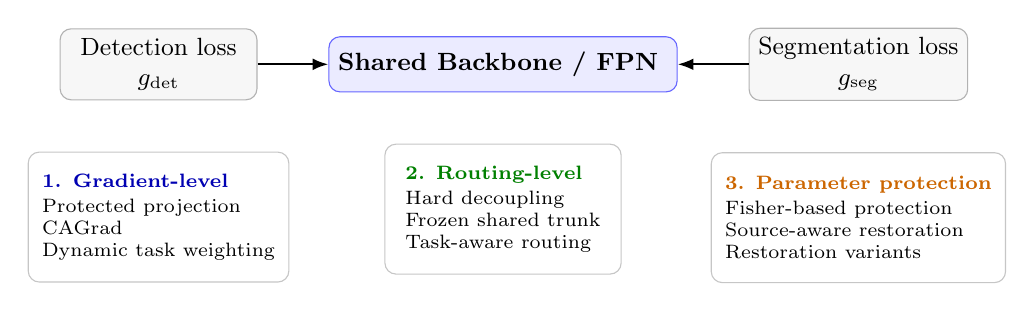
\begin{tikzpicture}[
    node distance=0.4cm and 0.7cm,
    task/.style={
        draw=gray!60,
        fill=gray!6,
        rounded corners,
        align=center,
        minimum width=2.5cm,
        minimum height=0.65cm,
        font=\small
    },
    trunk/.style={
        draw=blue!60,
        fill=blue!8,
        rounded corners,
        align=center,
        minimum width=2.8cm,
        minimum height=0.70cm,
        font=\small\bfseries
    },
    strategy/.style={
        draw=gray!45,
        fill=white,
        rounded corners,
        align=left,
        minimum width=3.0cm,
        minimum height=1.65cm,
        inner sep=5pt,
        font=\scriptsize
    },
    arr/.style={-{Latex[length=2mm]}, thick}
]

% Top row
\node[task] (det) {
Detection loss\\
$g_{\mathrm{det}}$
};

\node[trunk, right=0.9cm of det] (trunk) {
Shared Backbone / FPN
};

\node[task, right=0.9cm of trunk] (seg) {
Segmentation loss\\
$g_{\mathrm{seg}}$
};

\draw[arr] (det) -- (trunk);
\draw[arr] (seg) -- (trunk);

% Strategy boxes
\node[strategy, below=0.65cm of det] (grad) {
\textbf{\color{blue!70!black}1. Gradient-level}\\[1pt]
Protected projection\\
CAGrad\\
Dynamic task weighting
};

\node[strategy, below=0.65cm of trunk] (route) {
\textbf{\color{green!50!black}2. Routing-level}\\[1pt]
Hard decoupling\\
Frozen shared trunk\\
Task-aware routing
};

\node[strategy, below=0.65cm of seg] (protect) {
\textbf{\color{orange!80!black}3. Parameter protection}\\[1pt]
Fisher-based protection\\
Source-aware restoration\\
Restoration variants
};

\end{tikzpicture}%
}

\end{center}

\vspace{-0.2em}

\begin{block}{Questions tested}
\footnotesize
\begin{itemize}
    \setlength{\itemsep}{1pt}
    \setlength{\parskip}{0pt}
    \item Are conflicting task gradients the main source of damage?
    \item Should semantic gradients be restricted from the shared trunk?
    \item Can important source parameters be protected against continual drift?
\end{itemize}
\end{block}

\end{frame}

% -----------------------------------------------------------------------------

\begin{frame}{15. Semantic Drift and Shared-Trunk Routing}

\tiny
\setlength{\abovedisplayskip}{2pt}
\setlength{\belowdisplayskip}{2pt}
\setlength{\abovedisplayshortskip}{1pt}
\setlength{\belowdisplayshortskip}{1pt}

\textcolor{orange!80!black}{
\textbf{EARLIER SOURCE-MODEL CHECKPOINT --- DIAGNOSTIC ONLY}
}

\vspace{0.04cm}

\begin{columns}[T,onlytextwidth]

% ============================================================
% LEFT
% ============================================================
\begin{column}{0.46\textwidth}

\textbf{1. Semantic self-training drifts}

\[
\begin{aligned}
\text{Source} &= 31.66,\\
\text{Peak} &\approx 35.2 \;(\text{R4}),\\
\text{R10} &\approx 33.6
\end{aligned}
\]

% \vspace{-0.02cm}

Semantic adaptation helps initially, but part of the gain is lost
under prolonged continual exposure.

\vspace{0.08cm}

\textbf{Routing diagnostic}

\vspace{0.03cm}

\centering
\renewcommand{\arraystretch}{0.95}
\setlength{\tabcolsep}{3pt}

\begin{tabular}{lcc}
\toprule
\textbf{Config.} & \textbf{mAP50} & \textbf{mIoU} \\
\midrule
DET-only
& $26.93\pm0.20$
& $35.70\pm0.16$ \\
Routed SEG
& $26.76\pm0.14$
& $34.60\pm0.13$ \\
\bottomrule
\end{tabular}

\vspace{0.02cm}

{\fontsize{5.5}{6.2}\selectfont CSC diagnostic, 3 seeds}

\vspace{0.10cm}

\begin{block}{Takeaway}
\fontsize{5.7}{6.3}\selectfont
Semantic self-training shows residual temporal drift.
The shared semantic gradient is a plausible damage path.
\textbf{Routing helps diagnostically, but is not retained in the final method.}
\end{block}

\end{column}

% ============================================================
% RIGHT
% ============================================================
\begin{column}{0.51\textwidth}

\textbf{2. Where should gradients flow?}

\vspace{0.06cm}

\textbf{Full joint}

\[
\mathrm{DET}\rightarrow\boxed{\mathrm{trunk}}\rightarrow\mathrm{det}
\qquad
\mathrm{SEG}\rightarrow\boxed{\mathrm{trunk}}\rightarrow\mathrm{seg}
\]

Both tasks update the shared representation.

\vspace{0.05cm}

\textbf{Frozen trunk}

\[
\mathrm{DET}\rightarrow\mathrm{det}
\qquad
\mathrm{SEG}\rightarrow\mathrm{seg}
\]

The shared representation is fixed.

\vspace{0.05cm}

\textbf{Routed}

\[
\mathrm{DET}\rightarrow\boxed{\mathrm{trunk}}\rightarrow\mathrm{det}
\qquad
\mathrm{SEG}\rightarrow\mathrm{seg}
\]

Only detection updates the shared representation.

\vspace{0.08cm}

\textbf{Interpretation}

Routing nearly recovers the DET-only detection ceiling,
but blocking semantic gradients from the shared trunk also removes useful
shared plasticity.

\end{column}

\end{columns}

\end{frame}
% -----------------------------------------------------------------------------

\begin{frame}{16. CT-CR Robustness}

\fontsize{7.2}{7.8}\selectfont

\textbf{Is the CT-CR gain sensitive to its weight or to the stream order?}

\vspace{0.05cm}

\begin{columns}[T,onlytextwidth]

% ------------------------------------------------
% LEFT
% ------------------------------------------------
\begin{column}{0.56\textwidth}

\textbf{CT-CR weight sensitivity}

\vspace{0.02cm}

{\fontsize{6.7}{7.2}\selectfont Seed 0; short-term protocols}

\vspace{0.03cm}

\centering

\fontsize{6.6}{7.1}\selectfont
\setlength{\tabcolsep}{3.0pt}
\renewcommand{\arraystretch}{1.00}

\begin{tabular}{c|cc|cc}
\toprule
&
\multicolumn{2}{c|}{\textbf{CSC12}}
&
\multicolumn{2}{c}{\textbf{ACDC4}}
\\

$\lambda_{\mathrm{CTCR}}$
& mAP50 & mIoU
& mAP50 & mIoU
\\
\midrule

0.0
& 16.904
& 28.681
& 36.930
& 37.051
\\

0.1
& 17.504
& 29.543
& 37.401
& 37.207
\\

\textbf{0.3}$^{\star}$
& 17.840
& 30.278
& 38.367
& \textbf{37.773}
\\

0.5
& 17.980
& \textbf{30.430}
& \textbf{39.012}
& 37.673
\\

1.0
& \textbf{19.446}
& 29.734
& \multicolumn{2}{c}{\textit{diverged}}
\\

\bottomrule
\end{tabular}

\vspace{0.01cm}

{\fontsize{5.3}{5.8}\selectfont
$\star$ Selected operating point; bold values denote the best
non-diverged score in each metric.
}

\vspace{0.02cm}

\begin{block}{Weight choice}
\fontsize{5.6}{6.1}\selectfont
Increasing $\lambda_{\mathrm{CTCR}}$ can further improve individual metrics,
but a large weight becomes unstable on ACDC4.

Values $0.3$--$0.5$ provide strong gains across both domains.
We use \textbf{$\lambda_{\mathrm{CTCR}}=0.3$} as the conservative
cross-domain operating point rather than selecting a benchmark-specific optimum.
\end{block}

\end{column}

% ------------------------------------------------
% RIGHT
% ------------------------------------------------
\begin{column}{0.41\textwidth}

\textbf{Stream-order robustness}

\vspace{0.02cm}

{\fontsize{6.7}{7.2}\selectfont CSC12, seed 0; CT-CR vs.\ Base}

\vspace{0.05cm}

\centering

\fontsize{6.6}{7.1}\selectfont
\setlength{\tabcolsep}{3.5pt}
\renewcommand{\arraystretch}{1.03}

\begin{tabular}{lcc}
\toprule
\textbf{Order}
& $\Delta$mAP50
& $\Delta$mIoU
\\
\midrule

Canonical
& $+1.203$
& $+1.429$
\\

Reverse
& $+0.798$
& $+1.092$
\\

Random
& $+0.647$
& $+1.139$
\\

\bottomrule
\end{tabular}

\vspace{0.18cm}

\begin{block}{Observation}
\fontsize{5.6}{6.1}\selectfont
CT-CR improves both tasks under all three stream orders.

The magnitude changes, but the gain does not depend on one particular
corruption ordering.
\end{block}

\end{column}

\end{columns}

\vspace{-0.02cm}

\begin{block}{Takeaway}
\fontsize{6.0}{6.5}\selectfont
\textbf{CT-CR is not a narrowly tuned effect:}
the benefit persists across moderate loss weights and different
target-stream orders.
\end{block}

\end{frame}

\begin{frame}{17. Fisher-Based Source-Parameter Protection}

\footnotesize

\textbf{Hypothesis:}
parameters important for the source model should be protected more
strongly during continual adaptation.

\vspace{0.15em}

\begin{columns}[T,onlytextwidth]

% =====================================================
% LEFT COLUMN
% =====================================================
\begin{column}{0.45\textwidth}

\textbf{Parameter importance}

\vspace{0.1em}

A Fisher-style estimate assigns an importance score to each source
parameter:

\vspace{-0.25em}

\[
F_i
\approx
\mathbb{E}
\left[
\left(
\frac{\partial \log p(y|x;\theta)}
{\partial \theta_i}
\right)^2
\right]
\]

\vspace{-0.45em}

\begin{itemize}
    \setlength{\itemsep}{1pt}
    \setlength{\parskip}{0pt}
    \setlength{\parsep}{0pt}
    \item High $F_i$: source-sensitive parameter.
    \item Low $F_i$: more adaptable parameter.
\end{itemize}

\end{column}

% =====================================================
% RIGHT COLUMN
% =====================================================
\begin{column}{0.52\textwidth}

\textbf{Strategies explored}

\vspace{0.15em}

\textbf{\color{blue!70!black}Fisher-guided protection:}
protect or restore high-importance source parameters more strongly.

\vspace{0.3em}

\textbf{\color{blue!70!black}Cross-task Fisher variants:}
use parameter importance to reduce harmful updates through the shared
representation.

\vspace{0.3em}

\textbf{Conceptually:}

\vspace{-0.35em}

\[
\begin{aligned}
F_i \uparrow
&\Rightarrow \text{ stronger source protection},\\
F_i \downarrow
&\Rightarrow \text{ greater adaptation freedom}.
\end{aligned}
\]

\end{column}

\end{columns}

\vspace{-0.25em}

\begin{alertblock}{Result and takeaway}
\scriptsize
Fisher variants did not provide a consistent benefit over simpler
non-Fisher configurations.
Static source-parameter importance was therefore insufficient to solve
continual multi-task degradation, and Fisher-based variants were
\textbf{not retained in the final method}.
\end{alertblock}

\end{frame}


\begin{frame}{18. Task-CoCo: CAGrad-Style Gradient Coordination}

\scriptsize
\setlength{\abovedisplayskip}{3pt}
\setlength{\belowdisplayskip}{3pt}
\setlength{\abovedisplayshortskip}{2pt}
\setlength{\belowdisplayshortskip}{2pt}

\textbf{Goal:}
test whether explicit gradient-level coordination between detection and
segmentation improves over ordinary joint optimization.

\vspace{0.08cm}

\begin{columns}[T,onlytextwidth]

% ------------------------------------------------
% LEFT
% ------------------------------------------------
\begin{column}{0.48\textwidth}

\textbf{1. Native task gradients}

\[
g_{\mathrm{det}}
=
\nabla_{\theta_{\mathrm{sh}}}
\mathcal{L}_{\mathrm{det}},
\qquad
g_{\mathrm{seg}}
=
\nabla_{\theta_{\mathrm{sh}}}
\mathcal{L}_{\mathrm{seg}}.
\]

{\tiny
$\theta_{\mathrm{sh}}$: shared backbone / FPN parameters.
}

\vspace{0.08cm}

\textbf{2. Measure task interaction}

\[
G=
\begin{bmatrix}
\|g_{\mathrm{det}}\|^2
&
g_{\mathrm{det}}^\top g_{\mathrm{seg}}
\\
g_{\mathrm{seg}}^\top g_{\mathrm{det}}
&
\|g_{\mathrm{seg}}\|^2
\end{bmatrix}.
\]

\vspace{-0.08cm}

{\tiny
The off-diagonal term measures instantaneous task interaction:
positive $\rightarrow$ aligned,
negative $\rightarrow$ conflicting.
}

\end{column}

% ------------------------------------------------
% RIGHT
% ------------------------------------------------
\begin{column}{0.49\textwidth}

\textbf{3. CAGrad-style consensus search}

\[
\begin{aligned}
g_w
&=
w_{\mathrm{det}}g_{\mathrm{det}}
+
w_{\mathrm{seg}}g_{\mathrm{seg}},
\\
w&=\operatorname{softmax}(u),
\qquad
w_{\mathrm{det}}+w_{\mathrm{seg}}=1,
\\
g_0
&=
\frac{
g_{\mathrm{det}}+g_{\mathrm{seg}}
}{2}.
\end{aligned}
\]

\vspace{-0.05cm}

\[
w^*
=
\arg\min_w
\left[
g_w^\top g_0
+
\phi\|g_w\|_2
\right],
\qquad
\phi=c\|g_0\|_2.
\]

{\tiny
This is a task-specific application of the CAGrad-style
conflict-averse gradient coordination principle.
}

\end{column}

\end{columns}

\vspace{0.05cm}

\begin{block}{Shared-backbone update}
\vspace{-0.1cm}

\[
\boxed{
g_{\mathrm{shared}}
=
g_0
+
\frac{\phi}
{\|g_{w^*}\|_2+\epsilon}
\,g_{w^*}
+
g_{\mathrm{reg}}
}
\]

% \vspace{-0.15cm}

{\tiny
Task-CoCo coordinates only the native detection and segmentation gradients
on the shared backbone.
CT-CR, anchor stabilization, and other regularizers contribute normally
through $g_{\mathrm{reg}}$.
}
\end{block}

\vspace{-0.08cm}

{\tiny
\textbf{Key distinction:}
Task-CoCo = CAGrad-style gradient-level coordination;
CT-CR = explicit directional Det$\rightarrow$Seg supervision in prediction space.

\textit{Explored optimization variant; not retained in the final CTCMT configuration.}
}

\end{frame}

\begin{frame}{19. Final CTCMT Configuration}
\begin{block}{Final adaptation objective}
\[
\mathcal{L}_{\mathrm{CTCMT}}
=
\mathcal{L}_{\mathrm{det}}
+
\mathcal{L}_{\mathrm{seg}}
+
0.1\,\mathcal{L}_{\mathrm{anchor}}
+
0.3\,\mathcal{L}_{\mathrm{CTCR}}
\]
\end{block}


\begin{columns}[T]
\column{0.48\textwidth}
\textbf{Retained}
\begin{itemize}
  \item Detection pseudo-label adaptation
  \item Semantic soft consistency
  \item Frozen source anchor
  \item CT-CR
  \item EMA teacher
  \item Task-aware Stochastic restoration
  \item Class-balanced semantic consistency
\end{itemize}

\column{0.48\textwidth}
\textbf{Not retained}
\begin{itemize}
  \item CT-CL
  \item CTPV
  \item CAGrad / protected projection
  \item Fisher variants
  \item Special routing in the final method
  \item Task-CoCo
\end{itemize}
\end{columns}
\end{frame}


% -----------------------------------------------------------------------------

\begin{frame}{20. Short-Term Benchmark Comparison}

\scriptsize
\centering

\vspace{-0.12cm}

\setlength{\tabcolsep}{4.0pt}
\renewcommand{\arraystretch}{1.00}

\begin{tabular}{lcccc}
\toprule
&
\multicolumn{2}{c}{\textbf{ACDC4}}
&
\multicolumn{2}{c}{\textbf{CSC12}}
\\
\cmidrule(lr){2-3}
\cmidrule(lr){4-5}

\textbf{Method}
& \textbf{mAP50}
& \textbf{mIoU}
& \textbf{mAP50}
& \textbf{mIoU}
\\
\midrule

Source
& 34.084
& 35.211
& 13.457
& 27.602
\\

\midrule

\multicolumn{5}{l}{\textit{Single-task CTTA methods}} \\[-2pt]

AMROD
& 35.547
& --
& 15.788
& --
\\

CTAOD$^\ast$
& $\mathbf{38.788\pm0.126}$
& --
& $\mathbf{22.106\pm0.335}$
& --
\\

TENT-GN
& --
& 35.289
& --
& 27.257
\\

CoTTA
& --
& 34.376
& --
& 26.015
\\

OBAO-seg$^\dagger$
& --
& $\mathbf{38.249}$
& --
& 21.635
\\

DAT-BF$^\ddagger$
& --
& 36.221
& --
& 16.568
\\

\midrule

\multicolumn{5}{l}{\textit{Multi-task CTTA methods}} \\[-2pt]

Base
& $36.839\pm0.072$
& $36.864\pm0.172$
& $16.957\pm0.291$
& $28.948\pm0.665$
\\

CT-CR + Task-CoCo
& $37.749\pm0.315$
& $37.556\pm0.230$
& $17.267\pm0.328$
& $29.921\pm0.203$
\\

\textbf{CTCMT (Ours)}
& \underline{$38.007\pm0.254$}
& \underline{$37.800\pm0.064$}
& \underline{$17.722\pm0.264$}
& $\mathbf{30.073\pm0.189}$
\\

\bottomrule
\end{tabular}

\vspace{0.02cm}

{\fontsize{5.3}{5.9}\selectfont
\raggedright
``--'' = task not adapted/reported.
$^\ast$ CTAOD: 3 seeds.
$^\dagger$ OBAO-seg: seed 0, same-source segmentation port.
$^\ddagger$ DAT-BF: seed 0, same-source Panoptic-FPN port; not an official DAT reproduction.

Base, CT-CR + Task-CoCo and CTCMT: mean $\pm$ std over 3 seeds.
\par
}

\vspace{-0.04cm}

\begin{block}{Takeaway}
\fontsize{5.8}{6.4}\selectfont
Single-task methods can achieve the strongest score on one task,
whereas \textbf{CTCMT jointly adapts detection and segmentation}.
Compared with Base, CTCMT improves both tasks on both short-term protocols.
\end{block}

\end{frame}
% -----------------------------------------------------------------------------

\begin{frame}{21. Long-Term Benchmark Comparison}

\scriptsize
\centering

\vspace{-0.12cm}

\setlength{\tabcolsep}{4.0pt}
\renewcommand{\arraystretch}{1.00}

\begin{tabular}{lcccc}
\toprule
&
\multicolumn{2}{c}{\textbf{ACDC-LT}}
&
\multicolumn{2}{c}{\textbf{CSC-LT}}
\\
\cmidrule(lr){2-3}
\cmidrule(lr){4-5}

\textbf{Method}
& \textbf{mAP50}
& \textbf{mIoU}
& \textbf{mAP50}
& \textbf{mIoU}
\\
\midrule

% ------------------------------------------------
% SOURCE
% ------------------------------------------------
Source
& 34.084
& 35.211
& 14.469
& 28.940
\\

\midrule

% ------------------------------------------------
% SINGLE-TASK CTTA
% ------------------------------------------------
\multicolumn{5}{l}{\textit{Single-task CTTA methods}} \\[-2pt]

AMROD
& 38.744
& --
& 26.149
& --
\\

CTAOD$^\ast$
& 24.757
& --
& 13.640
& --
\\

TENT-GN
& --
& 35.469
& --
& 27.781
\\

CoTTA
& --
& 20.600
& --
& 26.731
\\

OBAO-seg$^\dagger$
& \textit{n/r}
& \textit{n/r}
& \textit{n/r}
& \textit{n/r}
\\

DAT-BF$^\ddagger$
& --
& 29.219
& --
& 13.798
\\

\midrule

% ------------------------------------------------
% MULTI-TASK CTTA
% ------------------------------------------------
\multicolumn{5}{l}{\textit{Multi-task CTTA methods}} \\[-2pt]

Base
& $42.494\pm0.090$
& $41.219\pm0.087$
& $25.266\pm0.511$
& $\mathbf{33.677\pm0.251}$
\\

CT-CR + Task-CoCo
& $43.369\pm0.129$
& $41.632\pm0.230$
& $25.806\pm0.299$
& $32.733\pm0.216$
\\

\textbf{CTCMT (Ours)}
& $\mathbf{44.076\pm0.357}$
& $\mathbf{41.921\pm0.256}$
& $\mathbf{26.725\pm0.463}$
& $33.334\pm0.320$
\\

\bottomrule
\end{tabular}

\vspace{0.02cm}

{\fontsize{5.2}{5.8}\selectfont
\raggedright

``--'' = task not adapted/reported; ``n/r'' = not run.
$^\ast$ CTAOD long-term: seed 0.
$^\dagger$ OBAO-seg: no long-term runs available.
$^\ddagger$ DAT-BF: seed 0, same-source Panoptic-FPN port; not an official DAT reproduction.

Base, CT-CR + Task-CoCo and CTCMT: mean $\pm$ std over 3 seeds.
\par
}

\vspace{-0.04cm}

\begin{block}{Takeaway}
\fontsize{5.8}{6.4}\selectfont
Under repeated exposure, \textbf{CTCMT achieves the highest mAP50 on both
long-term protocols} and the highest ACDC-LT mIoU.
On CSC-LT, Base remains slightly higher in segmentation
($33.677$ vs $33.334$), indicating a residual stability--plasticity trade-off.
\end{block}

\end{frame}

% \begin{frame}{Final Results: Cityscapes-C (CSC)}

% \scriptsize
% \centering

% \textit{Same canonical Cityscapes source model $\bullet$
% mAP50 detection / mIoU segmentation}

% \vspace{0.10cm}

% \setlength{\tabcolsep}{4.5pt}
% \renewcommand{\arraystretch}{1.10}

% \begin{tabular}{lcccc}
% \toprule
% &
% \multicolumn{2}{c}{\textbf{CSC12 (short-term)}}
% &
% \multicolumn{2}{c}{\textbf{CSC-LT (5 domains $\times$ 10 cycles)}}
% \\
% \cmidrule(lr){2-3}
% \cmidrule(lr){4-5}

% \textbf{Method}
% & \textbf{mAP50}
% & \textbf{mIoU}
% & \textbf{mAP50}
% & \textbf{mIoU}
% \\
% \midrule

% % ------------------------------------------------
% % SOURCE
% % ------------------------------------------------
% \multicolumn{5}{l}{\textit{Source model}} \\[-1pt]

% Source (no adaptation)
% & 13.457
% & 27.602
% & 14.469
% & 28.940
% \\

% \midrule

% % ------------------------------------------------
% % SINGLE-TASK CTTA
% % ------------------------------------------------
% \multicolumn{5}{l}{\textit{Single-task CTTA methods}} \\[-1pt]

% TENT-GN
% & \na
% & 27.257
% & \na
% & 27.781
% \\

% CoTTA
% & \na
% & 26.015
% & \na
% & 26.731
% \\

% OBAO-seg
% & \na
% & 21.635
% & \na
% & \na
% \\

% DAT-BF$^\ddagger$
% & \na
% & 16.568
% & \na
% & 13.798
% \\

% AMROD
% & 15.788
% & \na
% & 26.149
% & \na
% \\

% CTAOD$^\ast$
% & $\mathbf{22.106}\,{\tiny\pm0.335}$
% & \na
% & 13.639
% & \na
% \\

% \midrule

% % ------------------------------------------------
% % MULTI-TASK CTTA
% % ------------------------------------------------
% \multicolumn{5}{l}{\textit{Multi-task CTTA}} \\[-1pt]

% \textbf{CTCMT (Ours)}
% & $17.722\,{\tiny\pm0.264}$
% & $\mathbf{30.073}\,{\tiny\pm0.189}$
% & $\mathbf{26.725}\,{\tiny\pm0.463}$
% & $\mathbf{33.334}\,{\tiny\pm0.320}$
% \\

% \bottomrule
% \end{tabular}

% \vspace{0.18cm}

% {\tiny
% Bold = best value in each column.
% CTCMT: mean $\pm$ std over 3 seeds.
% $^\ast$CTAOD short-term: 3 seeds; CTAOD long-term: seed 0.
% All remaining adaptive baselines: seed 0.
% ``--'' denotes a task not adapted/reported by the corresponding method.
% }

% \vspace{0.05cm}

% \begin{block}{Takeaway}
% \tiny
% CTCMT achieves the best semantic segmentation performance in both CSC
% protocols and the best long-term detection performance.
% CTAOD remains stronger on short-term CSC12 detection.
% \end{block}

% \end{frame}

% \begin{frame}{Final Results: ACDC}

% \scriptsize
% \centering

% \textit{Same canonical Cityscapes source model $\bullet$
% mAP50 detection / mIoU segmentation}

% \vspace{0.10cm}

% \setlength{\tabcolsep}{4.5pt}
% \renewcommand{\arraystretch}{1.10}

% \begin{tabular}{lcccc}
% \toprule
% &
% \multicolumn{2}{c}{\textbf{ACDC4 (short-term)}}
% &
% \multicolumn{2}{c}{\textbf{ACDC-LT (4 domains $\times$ 10 cycles)}}
% \\
% \cmidrule(lr){2-3}
% \cmidrule(lr){4-5}

% \textbf{Method}
% & \textbf{mAP50}
% & \textbf{mIoU}
% & \textbf{mAP50}
% & \textbf{mIoU}
% \\
% \midrule

% % ------------------------------------------------
% % SOURCE
% % ------------------------------------------------
% \multicolumn{5}{l}{\textit{Source model}} \\[-1pt]

% Source (no adaptation)
% & 34.084
% & 35.211
% & 34.084
% & 35.211
% \\

% \midrule

% % ------------------------------------------------
% % SINGLE-TASK CTTA
% % ------------------------------------------------
% \multicolumn{5}{l}{\textit{Single-task CTTA methods}} \\[-1pt]

% TENT-GN
% & \na
% & 35.289
% & \na
% & 35.470
% \\

% CoTTA
% & \na
% & 34.376
% & \na
% & 20.600
% \\

% OBAO-seg
% & \na
% & $\mathbf{38.249}$
% & \na
% & \na
% \\

% DAT-BF$^\ddagger$
% & \na
% & 36.221
% & \na
% & 29.219
% \\

% AMROD
% & 35.547
% & \na
% & 38.744
% & \na
% \\

% CTAOD$^\ast$
% & $\mathbf{38.788}\,{\tiny\pm0.126}$
% & \na
% & 24.757
% & \na
% \\

% \midrule

% % ------------------------------------------------
% % MULTI-TASK CTTA
% % ------------------------------------------------
% \multicolumn{5}{l}{\textit{Multi-task CTTA}} \\[-1pt]

% \textbf{CTCMT (Ours)}
% & $38.007\,{\tiny\pm0.254}$
% & $37.800\,{\tiny\pm0.064}$
% & $\mathbf{44.076}\,{\tiny\pm0.357}$
% & $\mathbf{41.921}\,{\tiny\pm0.256}$
% \\

% \bottomrule
% \end{tabular}

% \vspace{0.18cm}

% {\tiny
% Bold = best value in each column.
% CTCMT: mean $\pm$ std over 3 seeds.
% $^\ast$CTAOD short-term: 3 seeds; CTAOD long-term: seed 0.
% All remaining adaptive baselines: seed 0.
% ``--'' denotes a task not adapted/reported by the corresponding method.
% }

% \vspace{0.05cm}

% \begin{block}{Takeaway}
% \tiny
% Single-task CTTA methods achieve the best individual short-term scores
% (CTAOD for detection and OBAO-seg for segmentation).
% Under repeated exposure, however,
% \textbf{CTCMT achieves the best performance on both tasks}.
% \end{block}

% \end{frame}

% \begin{frame}{Baseline Notes: Same-Source Comparison}

% \scriptsize

% \begin{itemize}
%   \setlength{\itemsep}{3pt}

%   \item All methods start from the same canonical
%   Panoptic-FPN R50 Cityscapes checkpoint
%   (MD5: \texttt{5f63c7578cb925552fd1b9d69980937a}).

%   \item Evaluation is strict online, batch size 1,
%   with no labels and no oracle/domain resets.

%   \item \textbf{TENT-GN, CoTTA, OBAO-seg and DAT-BF}
%   are segmentation-only CTTA methods;
%   \textbf{AMROD and CTAOD} are detection-only CTTA methods.

%   \item OBAO-seg and DAT-BF use the pre-update multi-view prediction;
%   TENT-GN, CoTTA and CTCMT report single-view post-update predictions.

%   \item CoTTA freezes stem/res2
%   (\texttt{FREEZE\_AT=2});
%   CoTTA and OBAO use stochastic parameter restoration,
%   while DAT-BF does not.

%   \item \textbf{DAT-BF} is a same-source Panoptic-FPN port,
%   not an official DAT reproduction:
%   whole-tensor selection, 10\% element cap,
%   no oracle domain boundaries.

%   \item Source-only segmentation was verified on the
%   \texttt{\_mtl} datasets, whereas TENT/CoTTA/DAT-BF use
%   \texttt{\_semseg}. Both use the same Cityscapes ground truth,
%   but source-only was not separately re-scored on
%   \texttt{\_semseg}.

%   \item CTCMT uses 3 seeds;
%   CTAOD short-term uses 3 seeds;
%   the remaining external baseline results are seed 0.
% \end{itemize}

% \end{frame}

% -----------------------------------------------------------------------------
\begin{comment}
    
\begin{frame}{22. Task-Specific Same-Source Baselines}

\scriptsize

\begin{columns}[T,onlytextwidth]

% ============================================================
% DETECTION
% ============================================================
\begin{column}{0.38\textwidth}

\textbf{Detection specialists}

\vspace{0.12cm}

\centering
\tiny
\setlength{\tabcolsep}{3.5pt}
\renewcommand{\arraystretch}{1.05}

\begin{tabular}{lcc}
\toprule
\textbf{Method}
& \textbf{CSC12}
& \textbf{ACDC4}
\\
& \textbf{AP50}
& \textbf{AP50}
\\
\midrule

AMROD
& 15.788
& 35.547
\\

CTAOD
& $22.106\pm0.335$
& $38.788\pm0.126$
\\

CTCMT
& $17.722\pm0.264$
& $38.007\pm0.254$
\\

\bottomrule
\end{tabular}

\vspace{0.18cm}

\raggedright
{\tiny
\textbf{CTAOD} is the stronger short-term detection specialist,
especially on CSC12.
}

\end{column}

% ============================================================
% SEGMENTATION
% ============================================================
\begin{column}{0.60\textwidth}

\textbf{Segmentation specialists}

\vspace{0.12cm}

\centering
\tiny
\setlength{\tabcolsep}{3.3pt}
\renewcommand{\arraystretch}{1.05}

\begin{tabular}{lcccc}
\toprule
\textbf{Method}
& \textbf{CSC12}
& \textbf{ACDC4}
& \textbf{CSC-LT}
& \textbf{ACDC-LT}
\\
& \textbf{mIoU}
& \textbf{mIoU}
& \textbf{mIoU}
& \textbf{mIoU}
\\
\midrule

CTCMT
& $30.073\pm0.189$
& $37.800\pm0.064$
& $33.334\pm0.320$
& $41.921\pm0.256$
\\

OBAO-seg$^\dagger$
& 21.635
& \textbf{38.249}
& -- & --
\\

DAT-BF$^\ddagger$
& 16.568
& 36.221
& 13.80
& 29.22
\\

\bottomrule
\end{tabular}

\vspace{0.14cm}

\raggedright
{\tiny
DAT-BF is only moderately useful on short-term ACDC4 and
\textbf{degrades strongly under repeated exposure}.
On ACDC-LT: roughly $37.1\rightarrow23.5$ mIoU from R1 to R10.
}

\end{column}

\end{columns}

\vspace{0.18cm}

{\tiny
$^\dagger$ OBAO-seg: seed 0; no long-term OBAO runs available.

$^\ddagger$ DAT-BF: seed 0; same-source Panoptic-FPN port,
not an official DAT reproduction.
}

\vspace{0.05cm}

\begin{block}{Takeaway}
\tiny
Task-specialized methods can win individual short-term settings,
but OBAO and DAT-BF are strongly benchmark-dependent.
CTCMT targets stable \textbf{joint OD+Seg adaptation} across both
short- and long-term protocols.
\end{block}

\end{frame}
\end{comment}

% -----------------------------------------------------------------------------
\begin{frame}{22. CTAOD: Short-Term Strength, Long-Term Drift}

\scriptsize

\begin{columns}[T,onlytextwidth]

% ------------------------------------------------
% LEFT COLUMN
% ------------------------------------------------
\begin{column}{0.44\textwidth}

\textbf{CSC-LT, seed 0}

\vspace{0.03em}

{\tiny
\begin{itemize}
    \setlength{\itemsep}{0pt}
    \setlength{\parskip}{0pt}
    \setlength{\parsep}{0pt}
    \setlength{\topsep}{1pt}
    \item CTAOD Round 1 mAP50: 24.34
    \item CTAOD Round 3 mAP50: 29.78
    \item CTAOD Round 6 mAP50: 7.24
    \item CTAOD Round 10 mAP50: 2.18
\end{itemize}
}

\vspace{-0.30em}

% Align table with list content
\hspace*{1.45em}
\begin{minipage}{0.72\linewidth}
\tiny
\setlength{\tabcolsep}{4pt}
\renewcommand{\arraystretch}{0.95}

\begin{tabular}{@{}lc@{}}
\toprule
\textbf{Method} & \textbf{mAP50} \\
\midrule
CTAOD (s0) & 13.64 \\
\textbf{CTCMT} & \textbf{26.725 $\pm$ 0.463} \\
\bottomrule
\end{tabular}
\end{minipage}

\end{column}

% ------------------------------------------------
% SPACE BETWEEN COLUMNS
% ------------------------------------------------
\hfill

% ------------------------------------------------
% RIGHT COLUMN
% ------------------------------------------------
\begin{column}{0.3\textwidth}

\textbf{ACDC-LT, seed 0}

\vspace{0.03em}

{\tiny
\begin{itemize}
    \setlength{\itemsep}{0pt}
    \setlength{\parskip}{0pt}
    \setlength{\parsep}{0pt}
    \setlength{\topsep}{1pt}
    \item CTAOD Round 1 mAP50: 38.76
    \item CTAOD Round 3 mAP50: 40.23
    \item CTAOD Round 6 mAP50: 24.62
    \item CTAOD Round 10 mAP50: 7.30
\end{itemize}
}

\vspace{-0.30em}

% Align table with list content
\hspace*{1.45em}
\begin{minipage}{0.72\linewidth}
\tiny
\setlength{\tabcolsep}{4pt}
\renewcommand{\arraystretch}{0.95}

\begin{tabular}{@{}lc@{}}
\toprule
\textbf{Method} & \textbf{mAP50} \\
\midrule
CTAOD (s0) & 24.76 \\
\textbf{CTCMT} & \textbf{44.076 $\pm$ 0.357} \\
\bottomrule
\end{tabular}
\end{minipage}

\end{column}

\end{columns}

\vspace{-0.70em}

\begin{center}
\includegraphics[
    width=0.82\textwidth,
    height=0.40\textheight,
    keepaspectratio
]{figures/ctaod_line_plot.png}
\end{center}

\vspace{-1.0em}

{\tiny
\centering
CTAOD long-term: seed 0
\qquad
CTCMT: mean $\pm$ std over 3 seeds.
\par
}

\vspace{-0.15em}

\begin{block}{Takeaway}
\tiny
CTAOD is strong in the first continual rounds, but
\textbf{degrades sharply under repeated exposure}.
CTCMT maintains substantially higher long-term mAP50 on both protocols.
\end{block}

\end{frame}

% -----------------------------------------------------------------------------

\begin{frame}{23. Efficiency}

\scriptsize
\centering

\textit{All timings measured on the same RTX 3090}

\vspace{0.08cm}

\setlength{\tabcolsep}{3.7pt}
\renewcommand{\arraystretch}{1.02}

\begin{tabular}{lcccc}
\toprule
\textbf{Method}
& \textbf{ms/frame}
& \textbf{FPS}
& \textbf{Peak mem.}
& \textbf{Overhead vs Base}
\\
\midrule

Base
& 620.6
& 1.61
& 5.88 GB
& -- \\

\textbf{CTCMT (plain joint)}
& \textbf{624.9}
& \textbf{1.60}
& \textbf{5.88 GB}
& \textbf{+0.7\%} \\

CT-CR + Task-CoCo
& 729.2
& 1.37
& 5.88 GB
& +17.5\% \\

CTCMT headline-run path$^\ast$
& 670.4
& 1.49
& 5.87 GB
& +8.0\% \\

\midrule

AMROD$^\dagger$
& 166.0
& 6.02
& 3.34 GB
& -- \\

CoTTA$^\dagger$
& 1386.3
& 0.72
& 5.54 GB
& -- \\

TENT-GN$^\dagger$
& 104.3
& 9.59
& 1.59 GB
& -- \\

\bottomrule
\end{tabular}

\vspace{0.05cm}

{\fontsize{5.3}{5.9}\selectfont
\raggedright
$^\ast$ Headline CTCMT experiments used the explicit
$\lambda_{\mathrm{route}}=1$ gradient-decomposition implementation.
At $\lambda_{\mathrm{route}}=1$, it produces the same update as ordinary
joint backpropagation, but incurs additional execution overhead.

$^\dagger$ AMROD is detection-only; CoTTA and TENT-GN are segmentation-only.
Their timings are shown for reference and are not direct workload-equivalent
comparisons with joint detection+segmentation CTTA.

CTCMT introduces no additional trainable parameters over Base.
\par
}

\vspace{-0.03cm}

\begin{block}{Key point}
\fontsize{5.8}{6.4}\selectfont
\textbf{CT-CR itself adds only $\sim$0.7\% runtime overhead}
and essentially no additional memory.
The observed $8\%$ headline-run overhead comes from an explicit
gradient-decomposition path that is \textbf{not required by the final method}.
\end{block}

\end{frame}
% -----------------------------------------------------------------------------

\begin{frame}{24. Baseline Status and Remaining Work}

\scriptsize

\begin{columns}[T,onlytextwidth]

% ------------------------------------------------
% LEFT
% ------------------------------------------------
\begin{column}{0.48\textwidth}

\textbf{Completed}

\begin{itemize}
    \setlength{\itemsep}{1pt}
    \item AMROD
    \item CTAOD:
          short-term $n=3$ + long-term seed 0
    \item TENT-GN / CoTTA same-source ports
    \item OBAO-seg:
          CSC12 + ACDC4, seed 0
    \item \textbf{DAT-BF: all four protocols, seed 0}
\end{itemize}

\end{column}

% ------------------------------------------------
% RIGHT
% ------------------------------------------------
\begin{column}{0.48\textwidth}

\textbf{Still open}

\begin{itemize}
    \setlength{\itemsep}{1pt}
    \item DAT-BF seeds 42 / 123
    \item OBAO official-code parity audit
    \item Final TENT / CoTTA baseline hygiene check
\end{itemize}

\vspace{0.1cm}

{\tiny
No OBAO long-term runs are currently available.
}

\end{column}

\end{columns}

\vspace{0.18cm}


\vspace{0.05cm}

\begin{block}{DAT-BF status}
\tiny
The same-source Panoptic-FPN DAT-BF port is
\textbf{weak overall}.
It is moderately useful on short-term ACDC4, but performs poorly on
CSC12 and degrades substantially under repeated exposure.
On ACDC-LT, mIoU falls from approximately
\textbf{37.1 at R1 to 23.5 at R10}.
\end{block}

\end{frame}
% -----------------------------------------------------------------------------
\begin{frame}{25. Conclusions}
\begin{enumerate}
  \item Joint OD+Seg continual test-time adaptation is feasible.
  \item Not every cross-task interaction is useful.
  \item CT-CL and CTPV were reasonable hypotheses but did not survive controlled ablation.
  \item Generic gradient surgery and Fisher protection did not consistently solve continual negative transfer.
  \item Directional \textbf{Detection $\rightarrow$ Segmentation CT-CR} is the strongest retained cross-task mechanism.
  \item The final method is intentionally simpler than the full design space explored.
\end{enumerate}

\vspace{0.5em}
\begin{center}
\Large\textbf{Exploit reliable cross-task structure without amplifying continual self-training errors.}
\end{center}
\end{frame}

% % -----------------------------------------------------------------------------
% \begin{frame}{27. Selected Related Methods}
% \small
% \begin{itemize}
%   \item CoTTA --- continual test-time adaptation with teacher consistency and augmentation averaging.
%   \item AMROD --- continual test-time adaptation for object detection.
%   \item CTAOD --- continual adaptation of object detectors.
%   \item OBAO --- continual semantic segmentation adaptation.
%   \item DAT --- distribution-aware continual semantic segmentation adaptation.
%   \item CAGrad --- conflict-averse gradient optimization for multi-task learning.
% \end{itemize}

% \vspace{0.5em}
% \textit{Add full bibliographic entries in the paper / final lab-meeting version.}
% \end{frame}

\end{document}
